%! TEX root = thesis.tex
% vim: ft=tex et sts=2 sw=2

\chapter{Introduction}

This dissertation discusses two problems that are more or less unrelated apart from having a common origin in soft-matter physics.
The concepts used for the discussion have their basis in a potpourri of fields ranging from classical and quantum mechanics to statistical mechanics to engineering, with an emphasis on geometric and asymptotic methods.

\section{Frameworks, thermal fluctuations, and free energy landscapes}

Simply put, a bar-joint mechanism is a deformable assembly of bars that connect freely rotating joints. Such mechanisms have served as highly idealized representations of mechanical structures that underlie a plethora of soft few-body systems, e.g., colloidal clusters, proteins, viruses, etc. More recently, DNA origami has made it possible to make these mechanisms at the nanoscale, where they undergo low-temperature thermal fluctuations due to the surrounding medium. Although the bars in a mechanism are only stiff and not rigid, it is useful to analyze a mecha- nism in the limit that the bars become fully rigid, i.e., when the bar lengths are fixed. Indeed, such a situation is an instance of a holonomically constrained classical system, often encountered in elementary mechanics.
However, the imposed holonomic constraints need not always be well-behaved.
To illustrate this point more generally, consider a particle constrained to move on two intersecting cylinders of equal radius with mutually perpendicular axes [Fig. 1(a)].
The configuration space of this particle is not a smooth manifold, precisely because the cylinders have a nontransversal intersection at two singular points, where they share a common tangent plane.
Such singularities, which arise when the constraints imposed on a system cease to be linearly independent, are not mere pathological irregularities, and they have been extensively studied in many fields, e.g., robotics and locomotion.

To shed some more light on the above discussion, consider a mechanical system with $n$ degrees of freedom, whose configuration at any given moment is fully described by a single configuration vector $\bm{q} \in \mathbb{R}^{n}$.
Constraints in such a system are most clearly introduced by defining a constraint map $f: \mathbb{R}^{n} \to \mathbb{R}^{m}$
that vanishes when the constraints are satisfied, where $m$ is the number of constraints introduced.
The map $f$ is a general nonlinear map in $\bm{q}$ and its linear approximation is given by the $m\times n$ Jacobian matrix $\nabla f$.
With these definitions, the configuration space of the system is $\Sigma = \left\{\bm{q} \in \mathbb{R}^{n} : f(\bm{q}) = \bm{0}\right\}$, which is the set of points where the constraints are satisfied exactly.
Furthermore, if the Jacobian $\nabla f$ has full rank for all points in $\Sigma$, standard theorems ensure that $\Sigma$ is a smooth $(n-m)$-dimensional manifold.%
\footnote{This condition is almost never explicitly stated in classical mechanics.
However, it is implicit in the oft-evoked argument that a mechanical system with $n$ degrees of freedom and $m$ constraints have $(n-m)$ degrees of freedom, with the configuration space $\Sigma$ parameterizable by $(n-m)$ generalized coordinates.}
At singularities, such as the ones in Fig.~XXX, the Jacobian drops rank, and $\Sigma$ fails to be a manifold,
which is another way of saying that the $m$ constraints cease to become linearly independent at these points.

In practice, there is no such thing as a system with perfect constraints, and it is always possible to violate them by paying some sort of an energy cost.
For realistic systems, the set $\Sigma$ would then form the ground-state manifold (assuming no other sources of energy).
At the most basic level, we can assume that energy $U$ of a stiffly constrained system depends only the value of the constraint map $f(\bm{q})$, so that we can take $U \equiv U[f(\bm{q})]$ with $U$ having a minimum for all points on $\Sigma$ where $f(\bm{q}) = \bm{0}$.

To see this at an even elementary level, assume that we have just one constraint so that the constraint map $f: \mathbb{R}^{n} \to \mathbb{R}$ and the Jacobian $\nabla f$ is just the gradient of $f$.
Taylor expanding the energy to $\mathcal{O}(\Abs{\bm{q}}^{2})$, we get the familiar Harmonic approximation result
%
\begin{equation}
  U[f(\bm{q})] \approx \tfrac{1}{2}U''\left[f(0)\right]\left(\nabla f\cdot \bm{q}\right)^{2}.
\end{equation}
%
Clearly, near points where $\nabla f$ vanishes (which is the equivalent of a rank-deficient Jacobian for a scalar map $f$) the harmonic approximation would give $U \approx 0$.
This shows that in the vicinity of points where $\nabla f$ becomes vanishingly small, we need to expand $U$ beyond the harmonic order for any meaningful description of the energy landscape.
Higher-order corrections to $U$ are usually weaker (after all $\Abs{\bm{q}}$ is assumed to be small), and consequently the system becomes energetically soft.
Although we restricted ourselves to the case with just one constraint here, the situation is analogous when there are more.



\section{Thin structures, elastic waves, and bound states}

\begin{figure}
  \begin{center}
    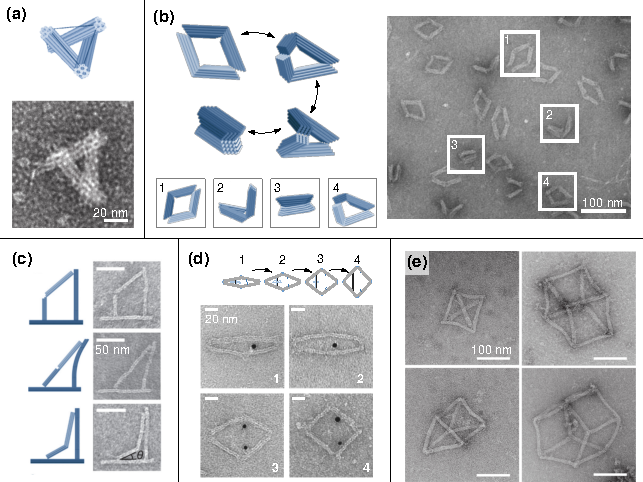
\includegraphics{dna.pdf}
  \end{center}
  \caption{DNA origami has been widely used to self assemble a variety of objects at the nanoscale.
    Depicted in the figure are (a) tensegrity structures \cite{liedl2010}; (b), (c) linkage-based mechanisms \cite{marras2015,zhou2015}; (d) a rhombus-shaped nanoactuator~\cite{ke2016}; and (e) self-assembled polyhedra~\cite{iinuma2014}.  All images used with permission.}
  \label{fig:dna_origami}
\end{figure}

\begin{figure}
  \begin{center}
    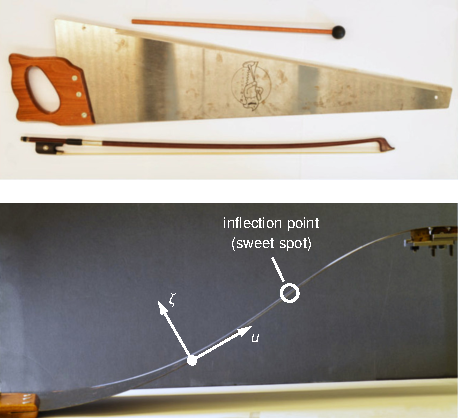
\includegraphics{saw/saw.pdf}
  \end{center}
  \caption{%
    An ordinary hand saw, when bent into the shape of the letter $\mathsf{S}$ can be played like a musical instrument using a violin's bow or a mallet.
    A sustained note is produced on bowing or hitting the saw at its inflection point, which is called a sweet spot by musicians.
    Photographs adapted from Ref.~\cite{shankar2022} and used with permission.
  }
  \label{fig:saw}
\end{figure}

\section{Organizational summary and other comments}

This dissertation is organized as follows:
Finally, in Appendix~\ref{app:math}, we collect some helpful mathematical results that are used throughout the dissertation.
